%\documentclass[11pt,aspectratio=169]{beamer}
\documentclass[11pt]{beamer}
\usetheme{Darmstadt}
%\usecolortheme{dolphin}

%\setbeameroption{show notes}
%\setbeameroption{show only notes}
%\usepackage{pgfpages}
%\pgfpagesuselayout{4 on 1}[a4paper]

\usepackage[utf8]{inputenc}
\usepackage[english]{babel}
\usepackage{amsmath}
\usepackage{amsfonts}
\usepackage{amssymb}
\usepackage{graphicx}
\usepackage{subcaption}
\usepackage{algorithmic}
\captionsetup{compatibility=false}

\title[D$^3$NS]{Distributed Decentralized Domain Name Service}
\author{
Brendan Benshoof \qquad Andrew Rosen  \qquad Anu G. Bourgeois \qquad Robert W. Harrison \\Department of Computer Science, Georgia State University\\ 25 Park Place\\ Atlanta, Georgia 30303\\  bbenshoof@cs.gsu.edu \qquad rosen@cs.gsu.edu  \qquad anu@cs.gsu.edu   \qquad rharrison@cs.gsu.edu }\author{Andrew Rosen}
\title[DHT Distributed Computing]{Proposal \\ Towards a Framework for DHT Distributed Computing}




\logo{
\includegraphics[height=1cm]{figs/logo}}
\institute{Georgia State University}
\date{May 27th, 2016}
%\subject{}
%\setbeamercovered{transparent}
%\setbeamertemplate{navigation symbols}{}



%\AtBeginSection[]
%{
%  \begin{frame}
%    \frametitle{Table of Contents}
%    \tiny{\tableofcontents[currentsection]}
%  \end{frame}
%}

\begin{document}
	
\maketitle

\section{Introduction}
\subsection{Motivation}

\begin{frame}{What is D$^3$NS}
Distributed Decentralized Domain Name Service

\begin{itemize}
	\item The goal is to create a secure distributed DNS. 
	\item Requirements 
	\begin{itemize}
		\item Decentralization
		\item Authentication
		\item Reliable
		\item No end user modification
	\end{itemize}
%	\item Requires distributed signing service for:
%	\begin{itemize}
%		\item Authentication
%		\item Thwarting man-in-the-middle attacks
%	\end{itemize}


\end{itemize}

\end{frame}



\begin{frame}{Motivation}
	\begin{itemize}
		\item  Recent events have demonstrated that centralized authorities are not as secure a previously hoped.
		\begin{itemize}
			\item There is little cryptographic protection against the subpoena.
			\item Poorly constructed laws targeting DNS.
		\end{itemize}	
		\item  A distributed approach for authentication is much less vulnerable.
	
	\end{itemize}
\end{frame}


\subsection{How We Built It}

\begin{frame}{Overview}

	\begin{itemize}
	
		\item Use a Distributed Hash Table (DHT) to organize a P2P network
		\begin{itemize}
			\item  UrDHT
		\end{itemize}
		\item Use a variant of NameCoin's blockchain to secure shared list of keys and domains.
		\item Use the DHT to load balance and distribute responsibility for hosting DNS
		and keys.
		\item DNS server frontend (PowerDNS)
	\end{itemize}
\end{frame}


\section{Components}

\subsection{DHTs}
%Cuttable
\begin{frame}{Distributed Hash Tables}

	\begin{itemize}
		\item  Means of organizing communication and responsibility in a P2P network
		\item  Each peer is responsible for a verifiable span of hash values
		\item  Facilitates one-to-one communication and one-to-many communication
	\end{itemize}

\end{frame}

\begin{frame}{UrDHT}
	\begin{itemize}
		\item Abstract DHT backend
		\item Handles:
		\begin{itemize}
			\item Organizing  nodes into a DHT or other DHTs
			\item Plugin Services
		\end{itemize}
		\item 
		\item Subject of other research
	\end{itemize}
\end{frame}

\begin{frame}{UrDHT Details}
% Cuttable
	\begin{itemize}
		\item DHT organization mechanism.
		
		\item Uses Voronoi regions on an $n$-dimensional torus to assign responsibility.
		\item Can define how to compute the regions to emulate almost any DHT topology.
		\item Node responsibility:
		\begin{itemize}
			\item Node is  responsible for its space, defined by its neighbors.
			\item If a node leaves/fails, each neighbors assumes that it is responsible until corrected by maintenance. 
		\end{itemize}
	\end{itemize}


\end{frame}

\begin{frame}{Fault Tolerance}
	\begin{itemize}
		\item Churn creates a period where i/o can fail.  With UrDHT:
		\item Reads of backed up data are successful.
		\item Writes to the region are successful. 
		\item Reads of new data are vulnerable until stabilization ($ <2$ sec currently).
		\item This means a much smaller window.  Writes never fail.\footnote{They may occur out of order}
		
	\end{itemize}


\end{frame}


\begin{frame}{Cool Thing UrDHT Can Do}
	\begin{itemize}
		\item Embed problem spaces into DHT topology
		\item Minimal latency based routing
		\item Basically turns routing into best-search first.
		
	\end{itemize}
\end{frame}


\subsection{Blockchain}
\begin{frame}{Blockchain}
% Cuttable
	\begin{itemize}
		\item Based on the blockchain verification of Bitcoin
		\item Allows for a shared, immutable and secure public records
		\item One block can include the validation of a new server's public key
		\item  One block can include a DNS record or change
		\item  Blocks require a proof of work to authenticate, causing records to be produced at a semi-fixed rate.
	\end{itemize}
\end{frame}

\begin{frame}{Blockchain}
	\begin{itemize}
		\item Using a technique similar to bitcoin, we can assign domain names as reward for mining new blocks and transfer domains between owners.
		
		\item An `owner' in this context is a public key
		
		\item These public keys can be used to verify stored DNS records by their signature
		records to be produced at a semi-fixed rate.
	\end{itemize}
\end{frame}




\begin{frame}
	\begin{figure}
	\centering
	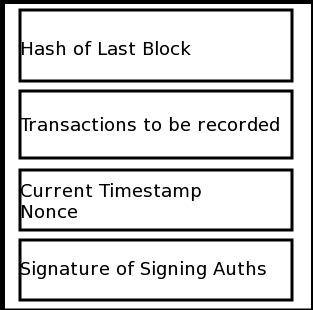
\includegraphics[width=0.4\linewidth]{namecoin_block}
	\caption{Contents of an individual block.}
	\label{fig:blockchain}
	\end{figure}

\end{frame}


\subsection{Frontend}
\begin{frame}{PowerDNS}
\begin{itemize}
	\item Well established authoritative DNS server software.
	
	\item Provides easy interface for custom applications.
	
\end{itemize}
\end{frame}

\section{Summary}

\subsection{Big Picture}

\begin{frame}{Current DNS}

	\begin{itemize}
		\item ICANN is the final arbiter on who owns what domain
		\item ICANN maintains and organizes the TLD authoritative name servers
		\item Third party verifiers act to authenticate DNS records
	
	\end{itemize}


\end{frame}



\begin{frame}{P2P-Based DNS}

	\begin{itemize}
		\item The shared block chain is the final arbiter of who owns what
		\item The DHT organizes and maintains the authoritative TLD servers
		\item The block chain acts to authenticate DNS records
	\end{itemize}


\end{frame}

\subsection{Security}

\begin{frame}{Man in the Middle In a DHT}

	\begin{itemize}
		\item Need to have a distributed, reliable way to authenticate 
		\item  Given: an existing network where nodes have exchanged keys securely
		\item  Given: a new peer who wishes to join the network and share their public key
	
	\end{itemize}


\end{frame}



\begin{frame}{Prevention}

	\begin{itemize}
		\item  At least 2 members of the network interrogate the new peer for its public key
		\item  Those interrogators compare their results
		\item  If those results match
		\begin{itemize}
		
		    \item The new peer creates an authentication record
		    \item The interrogators sign that record
		    \item The new record is distributed across the network
		\end{itemize}
		
		
		\item  If the results do not match
		\begin{itemize}
		
		    \item An attack is detected and reported to the new peer by all authenticating servers.
		    \item A member of the network may make a ban of the compromised peer
		    \item Otherwise the joining process can be repeated.
		\end{itemize}
		
	\end{itemize}


\end{frame}


\subsection{Conclusion}
\begin{frame}{Conclusions}
	\begin{itemize}
		\item 	Proof of concept of a decentralized and distributed top-level DNS.
		\item Fully reverse compatible.
		\item Offers greater security.
		\item Any organization can create their own secure verification server.
		
	\end{itemize}
\end{frame}



\section*{Appendix}
\begin{frame}{How Does This Differ From Namecoin?}
	\begin{itemize}
		\item Transparent to end users.
	\end{itemize}
\end{frame}


\end{document}
